As the users tend to move while using their phones, the generated CDR observations have semantics of trajectories. CDR data points can be grouped as trajectories so that the characteristics of trajectories and the result of previous research already conducted in this field can be utilized for achieving more accurate positioning.

We compare the ground truth GPS trajectories to trajectories of CDR events for the same time window in a distributed fashion as shown in Figure \ref{fig:problem}. 
\begin{figure}[h]
    \centering
    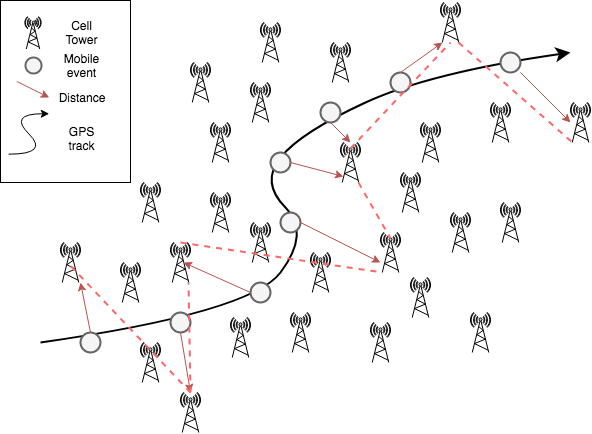
\includegraphics[width=0.45\textwidth]{images/problem.png}
    \caption{Problem illustration}
    \label{fig:problem}
\end{figure}

To evaluate cellular network event based customer localization we calculate the Euclidean distance and the DTW distance along with several statistics of the pairwise distances between ground truth GPS trajectories and mobile network event trajectories. The Haversine distance is used to define the spatial distance between points. In the mobile network event trajectory, the location information is obtained from cell map data set.

Similarly to the formulation in \cite{encyclopedia} and \cite{distance-def} we define distance measure on trajectories, such as:
\begin{definition}
Let $\mathcal{M}$ be a set of trajectories. A function $D :\mathcal{M} \times \mathcal{M} \rightarrow \mathcal{R}$ \nomenclature{$D$}{Distance measure defined on a set of trajectories.} is called a dissimilarity (distance) on $\mathcal{M}$ if for all $T_{1}, T_{2} \in \mathcal{M}$: 
\begin{itemize}
    \item $D(T_{1},T_{2}) \geqslant 0$
    \item $D(T_{1},T_{2}) = d(T_{2},T_{2})$
    \item $D(T_{1},T_{1}) = 0$
\end{itemize}
If all of these conditions are satisfied and $D(T_{1}, T_{2}) = 0 \Rightarrow  T_{1} = T_{2} $ is considered to be a symmetric. If
the triangle inequality is also satisfied, $D$ is a metric.
\end{definition}

The \textit{Euclidean distance} (or inverse similarity) measure between two trajectories is used in this analysis:
\[D(T,\Tilde{T}) = \sqrt{\sum_{i=1}^{n} (d(P_{i},\Tilde{P_{i}}))^{2}}\]

The Euclidean distance formula is implemented as presented in Algorithm \ref{algo:euclidean}.

\begin{algorithm}
\begin{algorithmic}
\caption{Euclidean distance function on trajectories} \label{algo:euclidean}
\Function{euclideanDist}{Traj tReal, Traj tApprox}
\State dEuclidean = 0
\State nPoints = len(tReal) 
\For{i \textbf{in} 0 to nPoints}
    \State dEuclidean = dEuclidean + power(haversine(     
    \State tReal[i], tApprox[i]) , 2)
\EndFor
\Return sqrt(dEuclidean)
\EndFunction
\end{algorithmic}
\end{algorithm}

The dynamic time warping distance is calculated similarly to the formulation given in \cite{traj-sim-rev}:
    \[
        D(T,\Tilde{T}) =
        \begin{cases}
            0, \text{if } n=m=0 \\
            \infty,\text{if }  n=0 \text{ or } m=0 \\
            d(h(T), h(\Tilde{T})) + \min 
            \begin{cases}  
                D(r(T),\Tilde{T}) \\
                D(T,r(\Tilde{T})) \\
                D(r(T),r(\Tilde{T})) 
            \end{cases}
        \end{cases}
    \]
where $h(.)$ returns the first point in the trajectory and $r(.)$ returns all except the first one.


\begin{algorithm}
\begin{algorithmic}
\caption{DTW distance function on trajectories} \label{algo:euclidean}
\Function{dtwDist}{Traj tReal, Traj tApprox}
    \If{(tReal is None) and (tApprox is None)} 
        \State\Return 0
    \EndIf
    \If{(tReal is None) or (tApprox is None)}
        \State\Return inf
    \EndIf

    \Return haversine(tReal.head(), tApprox.head()) + \State min(dtwDist(tReal, rest(tApprox)),     
    \State dtwDist(rest(tReal), tApprox), 
    \State dtwDist(rest(dReal), rest(dApprox)))
\EndFunction
\end{algorithmic}
\end{algorithm}

Given a set of distance observations with size $n$, we consider $\{d_{1}, d_{2}, ..., d_{n}\}$ as $n$ independent identically distributed (i.i.d) random variables, each corresponding to one randomly selected observation and having the distribution of the population. Then we can calculate the following descriptive statistics for the sample:
\begin{itemize}
    \item mean:
     \[ \overline {d} = \frac{\sum_{i=1}^{n} d_{i}}{n}\]
     \item standard deviation:
    \[ \sigma={\sqrt {\frac {\sum _{i=1}^{n}(d_{i}-{\overline {d}})^{2}}{n-1}}}\]
    \item sum:        
    \[s = \sum_{i=1}^{n} d_{i}\]
\end{itemize}

Note that $\{d_{1}, d_{2}, ..., d_{n}\}$ are the spatial distances between pairs of points from the trajectories. For each pair of points, $d_{i} = d(P_{i},\Tilde{P_{i}})$ and $n$ is the number of points in the trajectories.

For calculation of the descriptive statistics and the Euclidean distance the number of CDR and GPS observations need to match, which by the design of the data collection is guaranteed.

In this paper we do not attempt to reconstruct trajectories from CDR data considering the road network of Berlin. Instead we consider the sequence of positioned mobile network events together with the GPS observation and we try to determine the distance of the two trajectories based on the distances of individual pairs of points.



